\documentclass[12pt, a4paper]{article}

\usepackage[czech]{babel}
\usepackage[IL2]{fontenc}
\usepackage[utf8]{inputenc}
\usepackage{lmodern}  % lepší kvalita PDF

\usepackage[a4paper,top=3cm,bottom=3cm,left=3cm,right=3cm,marginparwidth=1.75cm]{geometry}

\usepackage{graphicx}
\usepackage{titling}
\usepackage[colorlinks=true, allcolors=black]{hyperref}
\usepackage{url}
\usepackage{enumitem}

% vlastní příkazy
\newcommand{\lt}{\textless}
\newcommand{\gt}{\textgreater}

\title{Webová aplikace programátorské konference}
\def \thesubtitle {Semestrální práce z předmětu KIV/WEB}
\author{Patrik Harag}
\def \theauthoremail {harag@students.zcu.cz}
\def \theauthorid {(A15B0034P)}

\begin{document}

% titulní strana
\begin{titlepage}
	\begin{figure}
		
\includegraphics[height=50mm]{img-fav-logo}
	\end{figure}
	
	\centering
	{\large \hspace{1mm} \par} % tady musí být nějaký text jinak nefunguje vertikální odsazení
	\vspace{15ex}
	
	{\scshape\Large \thesubtitle \par}
	\vspace{1.5ex}
	{\huge\bfseries \thetitle \par}
	\vspace{2ex}
	{\Large\itshape \theauthor \par}
	\vspace{2ex}
	{\texttt{\theauthoremail} \par}
	\vspace{1ex}
	{\texttt{\theauthorid} \par}
	
	\vfill
	
	{\large \today\par}
\end{titlepage}

% strana s obsahem
%\setcounter{page}{0} 
%\tableofcontents
%\thispagestyle{empty}


\section{Použité technologie}
\begin{description}
	\item [Apache + PHP + MariaDB (WAMP)]
	\item [Twig] Šablonovací systém. Každá stránka využívá nějakou šablonu. Šablony tvoří hierarchii.
	\item [Bootstrap] \emph{Front-end} framework. Využíván je především pro vzhled, layout, ovládací prvky, formuláře, dialogy\dots
	\item [JavaScript + jQuery] Použité pro větší interaktivitu webových stránek (např. počítadlo zbývajících znaků), nezbytné pro inicializaci některých ovládacích prvků (např. dialogy). \emph{jQuerry} je také závislostí dalších použitých technologií.
	\item [AJAX] Použit pro kontrolu dostupnosti uživatelského při registraci.
	\item [starrr] Mini knihovna přidávající komponentu pro hodnocení hvězdičkami. Recenzenti pomocí této komponenty hodnotí publikace.
	\item [Font Awesome] Umožňuje vkládání vektorových ikon do webu. Použito hlavně kvůli ikoně hvězdičky.
	\item [CKEditor] Jedná se o \emph{WYSIWYG} HTML editor. Administrátor může pomocí tohoto editoru upravovat obsahové stránky.
\end{description}


\section{Popis adresářové struktury}
\begin{itemize}
	\item \emph{lib} -- obsahuje knihovny a další závislosti. Projekt nemá žádné externí závislosti, vše potřebné je zde.
	\item \emph{model} -- vrstva pracující s databází a obsahující doménovou logiku.
	\item \emph{view}
	\begin{itemize}[label=$\bullet$]
		\item \emph{templates} -- obsahuje šablony napsané v šablonovacím systému \emph{Twig}.
		\item \emph{css} -- obsahuje kaskádové styly.
		\item \emph{resources} -- obsahuje obrázky. Případně by obsahoval i jiná potřebná data.
	\end{itemize}
	\item \emph{controller} -- obsahuje kontrolery pro všechny stránky.
\end{itemize}

\pagebreak

\section{Architektura aplikace}
Webová aplikace se striktně drží architektury MVC.

\subsection{Model}
\emph{Model} pracuje s databází a obsahuje doménovou logiku. Ostatním částem aplikace poskytuje API, pomocí kterého mohou manipulovat s daty. \\

\noindent
Pro každý typ dat \emph{model} poskytuje neměnnou třídu:
\begin{itemize}
	\item \emph{Article}
	\item \emph{User}
	\item \emph{Publication}
	\item \emph{Review}
	\item \emph{Comment}
\end{itemize}

\pagebreak[2]

\noindent
Ke každé takové třídě se váže třída obsahující statické metody pro práci s tímto typem dat:
\begin{itemize}
	\item \emph{Articles}
	\item \emph{Users}
	\item \emph{Publications}
	\item \emph{Reviews}
	\item \emph{Comments}
\end{itemize}
Například \emph{Users::loadAllUsers()} načte všechny uživatele jako kolekci typů \emph{User}. Třídy \emph{User} a \emph{Users} jsou pro jednoduchost a snadné použití uloženy v jedné třídě nazvané \emph{users.php}. A podobně ostatní třídy\dots

\emph{Model} dále obsahuje třídu zajišťující spojení s databází a třídu pro kontrolu přihlášení uživatele.

\begin{figure}
	\centering
	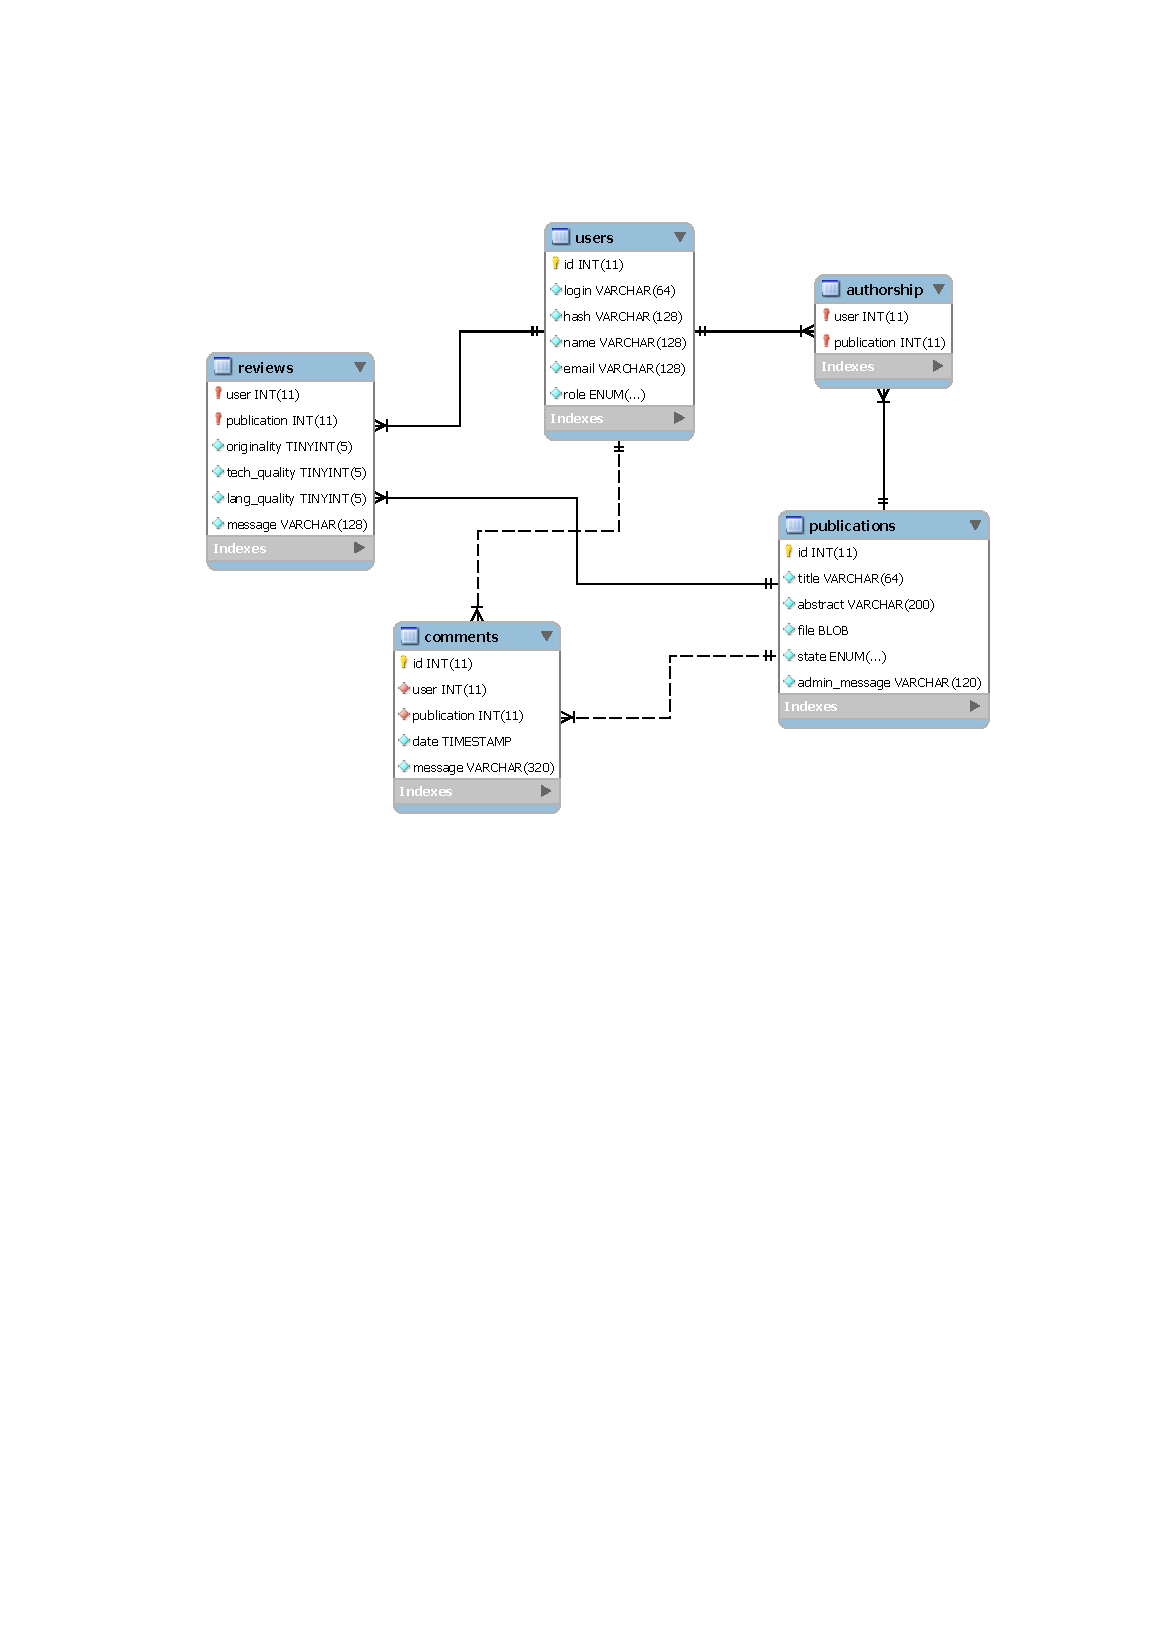
\includegraphics[width=1.2\linewidth,trim={3cm 13cm 0 3cm},clip]{schema}
	\caption{ER diagram databázové vrstvy.}
	\label{fig:schema}
\end{figure}


\subsection{View}
\emph{View} zahrnuje v podstatě jen šablony a \emph{CSS}.

Základní šablonou je \emph{layout.twig}, která definuje rozložení a vzhled stránky. Ostatní šablony od ní dědí a definují pouze obsah článku.

Šablonám jsou často předávány datové třídy z modelu. \emph{Twig} totiž dokáže pracovat s třídami stejným způsobem jako s poli, kdy není nutné psát počáteční \emph{get} a závorky, ale jen název příslušné \emph{property}. Nevzniká tak žádná závislost.

\subsection{Controller}
Zahrnuje hlavní kontroler v souboru \emph{index.php} a kontrolery jednotlivých stránek, které jsou všechny třídy, dědící od \emph{Page}. 

Hlavní kontroler podle parametru \emph{page} předaným metodou \emph{GET} nebo \emph{POST} vybere příslušnou třídu a vytvoří její instanci. Otestuje, zda má uživatel právo přístupu k této stránce, prostřednictvím metody \emph{hasAccess(\$user)}, a poté ji zobrazí metodou \emph{show()}. Pokud uživatel nemá právo přístupu, zobrazí jinou stránku.

Kontrolery jednotlivých stránek v zásadě jen (částečně) validují vstupy, předávají vstupy modelu a data získaná z modelu nechají zobrazit pomocí šablony nebo po předání dat modelu přesměrují na jinou stránku.


\section{Závěr}
Vytvořili jsme fungující webovou aplikaci programátorské konference. Aplikace je navržena spíše pro menší počet uživatelů. Pro větší počet uživatelů by bylo nutné upravit webové rozhraní tak, aby bylo možné rozumně pracovat i s většími daty (například filtrování, načítání jen části záznamů\dots). \\

\noindent
Repozitář s projektem:

\url{https://github.com/Hartrik/KIV-WEB}

\end{document}